\documentclass[tikz,border=12pt]{standalone}
\usepackage{fontspec}
\setmainfont{Segoe UI}
\usepackage{amsmath,amssymb}
\usepackage{tikz}

\usetikzlibrary{calc,arrows.meta}

\begin{document}
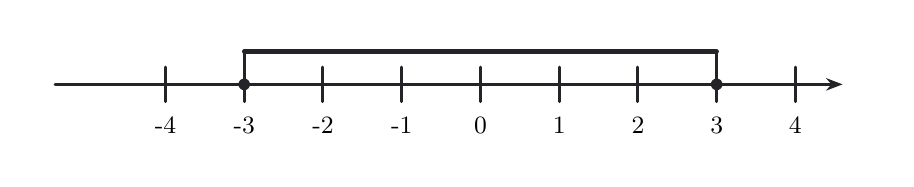
\begin{tikzpicture}[x=1.0000cm,y=1cm,line cap=round,line join=round]
\definecolor{linec0}{RGB}{35,35,40}
\definecolor{linec1}{RGB}{35,35,40}
\definecolor{linec2}{RGB}{35,35,40}
\definecolor{linec3}{RGB}{35,35,40}
\definecolor{linec4}{RGB}{35,35,40}
\definecolor{linec5}{RGB}{35,35,40}
\definecolor{edgecol}{RGB}{35,35,40}
\definecolor{hicol}{RGB}{35,35,40}
\definecolor{angcol}{RGB}{35,35,40}
\coordinate (L) at (-5.4000,0.0000);
\coordinate (R) at (4.6000,0.0000);
\coordinate (A) at (-3.0000,0.0000);
\coordinate (B) at (3.0000,0.0000);
\coordinate (S) at (-3.0000,0.4200);
\coordinate (T) at (3.0000,0.4200);
\draw[edgecol,line width=1.1pt,-{Stealth[length=2.1mm]}] (L) -- (R);
\draw[hicol,line width=1.6pt] (S) -- (T);
\draw[edgecol,line width=1.1pt] (S) -- (A);
\draw[edgecol,line width=1.1pt] (T) -- (B);
\fill[edgecol] (A) circle [radius=2.1pt];
\fill[edgecol] (B) circle [radius=2.1pt];
\draw[edgecol,line width=1.05pt] (-4.000,-0.220) -- (-4.000,0.220);
\node[anchor=north,inner sep=1pt,font=\small] at (-4.000,-0.380) {-4};
\draw[edgecol,line width=1.05pt] (-3.000,-0.220) -- (-3.000,0.220);
\node[anchor=north,inner sep=1pt,font=\small] at (-3.000,-0.380) {-3};
\draw[edgecol,line width=1.05pt] (-2.000,-0.220) -- (-2.000,0.220);
\node[anchor=north,inner sep=1pt,font=\small] at (-2.000,-0.380) {-2};
\draw[edgecol,line width=1.05pt] (-1.000,-0.220) -- (-1.000,0.220);
\node[anchor=north,inner sep=1pt,font=\small] at (-1.000,-0.380) {-1};
\draw[edgecol,line width=1.05pt] (0.000,-0.220) -- (0.000,0.220);
\node[anchor=north,inner sep=1pt,font=\small] at (0.000,-0.380) {0};
\draw[edgecol,line width=1.05pt] (1.000,-0.220) -- (1.000,0.220);
\node[anchor=north,inner sep=1pt,font=\small] at (1.000,-0.380) {1};
\draw[edgecol,line width=1.05pt] (2.000,-0.220) -- (2.000,0.220);
\node[anchor=north,inner sep=1pt,font=\small] at (2.000,-0.380) {2};
\draw[edgecol,line width=1.05pt] (3.000,-0.220) -- (3.000,0.220);
\node[anchor=north,inner sep=1pt,font=\small] at (3.000,-0.380) {3};
\draw[edgecol,line width=1.05pt] (4.000,-0.220) -- (4.000,0.220);
\node[anchor=north,inner sep=1pt,font=\small] at (4.000,-0.380) {4};
\path (-5.750,-0.950) rectangle (5.150,0.720);
\end{tikzpicture}
\end{document}
